% ==================================================================
\section{问题一：原始视频的三模态特征与时间对齐}\label{sec:q1}
% ==================================================================

问题一要从100段原始视频得到固定长度的三模态特征，并让每个位置都能回到原始的词、声学帧和视频帧。本章先给出词级时间的求法，再给出三路特征的构造和池化规则，最后用一条典型样本和全量台账检验结果。需要强调的是，本章的目标是构造可以逐条核对的原始数据映射，而不是去模仿附件2特征的数值；问题二的模型也不在这些特征上训练。

\subsection{原始样本与处理流程}

附件1的100段视频来自37个源视频，以二元组 $i=(\text{video\_id},\text{clip\_id})$ 唯一标识。转写文本和情感标签一律取自题目给定的 label-100.xlsx，不用自动语音识别的结果替换原文。每段视频先用 ffprobe 读取时长 $D_i$，再用 ffmpeg 抽出16 kHz 单声道音频。按 ffprobe 的读数，100段时长在2.257～29.288秒之间，合计约787秒；这一范围与赛题说明中给出的2.648～34.567秒不完全一致，本文以实际文件的读数为准。

整条处理链分三步：先求词级时间（第\ref{sec:q1time}节），再把声学帧和视觉帧按词时间窗池化到子词位置（第\ref{sec:q1feat}节），最后为每个位置记录能否观测以及失败原因（第\ref{sec:q1mask}节）。三步完成后，每个有效位置都挂着一条“原文字符 $\to$ 词 $\to$ 子词位置 $\to$ 音视频帧”的反查链。

\subsection{词级时间映射}\label{sec:q1time}

以视频起点为零时刻，把原转写按非空白字符切成词 $w_{ij}$，同时保存每个词在原文中的字符区间 $[c_{ij},d_{ij})$。WhisperX\cite{bain2023whisperx} 对给定转写做强制对齐，求出每个词的起止时间。首轮没有全部对齐成功时，程序会利用静音边界把句子切开后重新对齐；静音边界只用来辅助切句，不作为最终的词时间，我们也不用均匀切分去补造时间。规范化词串匹配以后，只对拿到有效数值区间的词记录 $[s_{ij},e_{ij})$。

文本用冻结的 bert-base-uncased 取最后一层隐状态\cite{devlin2019bert}。WordPiece 编码加上 \texttt{[CLS]} 和 \texttt{[SEP]} 后长度固定为50，最多保留48个正文子词，不足的位置补齐。设位置 $p$ 的子词在原文中的字符区间为 $[u_{ip},v_{ip})$，按字符重叠最大的原则确定它属于哪个原词：
\begin{equation}\label{eq:overlap}
j_i(p)=\mathop{\arg\max}_{j:\ [u_{ip},v_{ip})\cap[c_{ij},d_{ij})\neq\varnothing}\ \big|[u_{ip},v_{ip})\cap[c_{ij},d_{ij})\big|.
\end{equation}
如果某个位置和任何原词都没有重叠，或者对应的词没有有效时间，就保留这个位置和原因，但不给它写入音视频时间。\texttt{[CLS]}、\texttt{[SEP]} 和补齐位也不冒充任何词。文本矩阵 $X_i^T\in\mathbb{R}^{50\times768}$ 的补齐行置零，同时保存词元编号、注意力掩码和分段编号。

\subsection{声学与视觉特征及词窗池化}\label{sec:q1feat}

声学特征用 openSMILE\cite{eyben2010opensmile} 的 eGeMAPSv02 低层描述量，共25维\cite{eyben2016gemaps}，包括音高、响度、共振峰、频谱斜率等与情感表达关系密切的量。视觉特征用 OpenFace 2.0\cite{baltrusaitis2018openface} 的人脸动作单元（AU），其中17维是强度、18维是出现标志，共35维；动作单元直接对应皱眉、嘴角上扬这类面部动作，比笼统的人脸框统计量更贴近表情。

声学帧的时刻取其时间窗的中点 $\tau_{ik}^A$，视频帧的时刻取 OpenFace 给出的时间戳 $\tau_{ik}^V$。视觉帧必须同时满足三个条件才算有效：提取成功、置信度不低于0.8、数值有限。设 $\boldsymbol z_{ik}^m$ 为模态 $m\in\{A,V\}$ 的第 $k$ 帧向量，$b_{ik}^m$ 为其有效标志，则位置 $p$ 的池化帧集合与特征为
\begin{equation}\label{eq:pool}
\mathcal{I}_{ip}^m=\big\{k:\ s_{i,j_i(p)}\le\tau_{ik}^m<e_{i,j_i(p)},\ b_{ik}^m=1\big\},\qquad
\boldsymbol x_{ip}^m=\begin{cases}\dfrac{1}{|\mathcal{I}_{ip}^m|}\displaystyle\sum_{k\in\mathcal{I}_{ip}^m}\boldsymbol z_{ik}^m, & |\mathcal{I}_{ip}^m|>0,\\[10pt]\mathbf{0}, & |\mathcal{I}_{ip}^m|=0.\end{cases}
\end{equation}

同一个词切出的几个子词继承同一个词时间窗，因此会引用同一批声学帧和视频帧。这是有意为之：它们本来就是同一个词，时间上不该被人为拆开；但也要注意，这几个位置并不是几次独立的观测。最终得到 $X_i^A\in\mathbb{R}^{50\times25}$、$X_i^V\in\mathbb{R}^{50\times35}$，并为每个有效位置保存声学帧数、视频起止帧号和原始秒数。

\subsection{可观测状态与有效长度}\label{sec:q1mask}

零值本身说明不了“这里没有表情”还是“这里没提取到”，所以我们为每个位置单独记录可观测状态。令 $\ell_{ip}$ 为注意力掩码、$h_{ip}$ 为特殊词元标志，则文本可观测位 $o_{ip}^T=\ell_{ip}(1-h_{ip})$，声学、视觉可观测位 $o_{ip}^m=\mathbb{1}\{|\mathcal{I}_{ip}^m|>0\}$。各模态的有效长度为
\begin{equation}\label{eq:len}
L_i^m=\sum_{p=0}^{49}o_{ip}^m,\qquad m\in\{T,A,V\}.
\end{equation}
下游读取特征时必须同时读取掩码，不能把矩阵里的零解释为真实的静音或面无表情。如果某个模态在提取阶段就失败了，根本没有生成矩阵，文件里记为 None，与“矩阵存在但某些位置为零”区分开。三路特征的存储接口见表\ref{tab:q1io}。

\begin{table}[htbp]
\centering
\caption{问题一自提特征的存储接口（有效位置数均按可观测掩码计）}
\label{tab:q1io}
\begin{tabularx}{\textwidth}{l>{\raggedright\arraybackslash}Xc>{\raggedright\arraybackslash}X}
\toprule
模态 & 原始依据与提取器 & 单样本矩阵 & 有效位置与反查字段 \\
\midrule
文本 & 给定转写；冻结 BERT，WordPiece & $50\times768$ & 正文子词；字符区间、原词 \\
声学 & 16 kHz 音频；eGeMAPSv02 低层描述量 & $50\times25$ & 词窗内帧；秒数、帧数 \\
视觉 & 原视频；OpenFace 动作单元 & $50\times35$ & 达标动作单元帧；秒数、视频帧号 \\
\bottomrule
\end{tabularx}
\end{table}

\subsection{典型样本验证}\label{sec:q1case}

我们从人工核验表中选了样本 \texttt{-3g5yACwYnA\$\_\$13}。它的原句是 \textit{They've been able to find solutions or at least bring some answers to the table.}，视频时长5.514秒，15个词全部拿到了时间，18个正文子词的文本、声学、视觉位置都可观测。表\ref{tab:q1case}列出了句首五个词在三路上的对应关系。

\begin{table}[htbp]
\centering
\caption{样本 \texttt{-3g5yACwYnA\$\_\$13} 句首五词的“词—秒—帧—位置”对应（取自 q1\_alignment.csv）}
\label{tab:q1case}
\begin{tabular}{lcccc}
\toprule
原词 & 视频时间/s & 文本位置 & 声学帧数 & 有效视频帧号 \\
\midrule
They've & 1.445–1.586 & 1–3 & 14 & 45–48 \\
been & 1.606–1.726 & 4 & 12 & 50–52 \\
able & 1.746–1.927 & 5 & 18 & 54–58 \\
to & 1.967–2.067 & 6 & 10 & 60–62 \\
find & 2.148–2.409 & 7 & 26 & 66–73 \\
\bottomrule
\end{tabular}
\end{table}

这张表可以直接用来核对。以 They've 为例，它被 BERT 切成3个子词，占第1～3个位置，三个位置共用同一个词时间窗，因而共用同样的14个声学帧和第45～48号视频帧。声学帧数也和时长对得上：帧移10毫秒，0.141秒的词窗恰好约14帧；其余四个词同样如此。表中所列15个词的核验结果都是通过。图\ref{fig:q1case}把这条样本的50个位置与三路特征并排画了出来。

\begin{figure}[htbp]
\centering
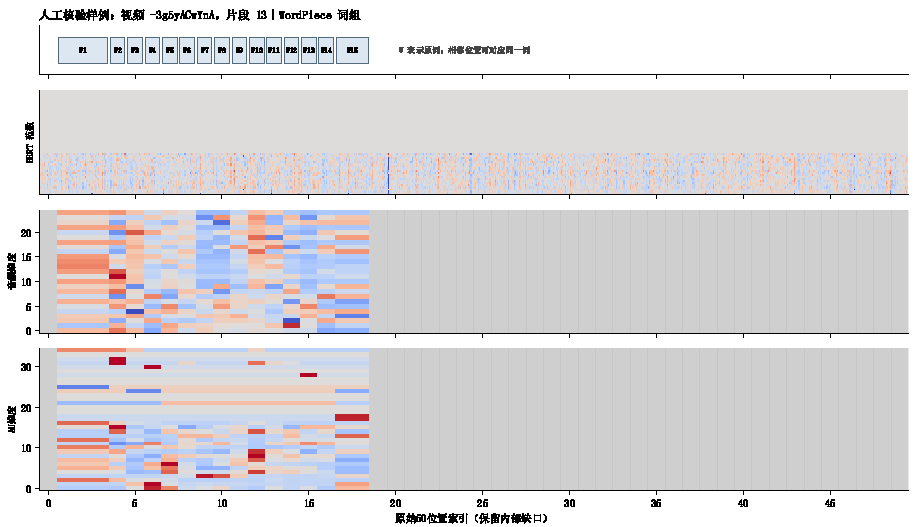
\includegraphics[width=\textwidth]{figures/fig_q1_sample.pdf}
\caption{样本 \texttt{-3g5yACwYnA\$\_\$13} 的位置—时间映射与三路观测。最上一行用 W 编号标出原词，相邻的几个子词可对应同一个词；灰色表示该模态在该位置没有有效观测。声学与动作单元热图按本样本的可观测位置逐维标准化并截断到 $[-3,3]$，只用于展示结构}
\label{fig:q1case}
\end{figure}

图中能看出两个特点。一是三路的有效区间完全对齐，都在前18个正文位置上，之后是整齐的补齐区；二是声学和动作单元热图的第1～3列颜色完全相同，这就是 They've 的三个子词共享同一个词时间窗的直接体现。

\subsection{全量结果与异常核验}\label{sec:q1res}

100条样本的逐条台账见附录\ref{app:A}的表\ref{tab:appA}，包括时长 $D_i$、三个有效长度、词级对齐成功数 $W_i$（拿到时间的词数/原词总数）、处理状态和截断标志。图\ref{fig:q1status}给出了全量的处理状态、对齐分支和有效长度分布。

\begin{figure}[htbp]
\centering
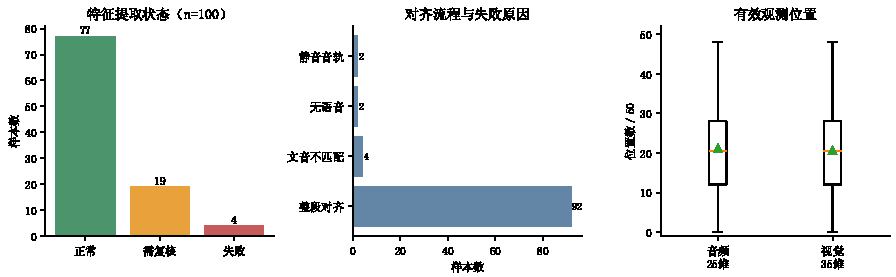
\includegraphics[width=\textwidth]{figures/fig_q1_status.pdf}
\caption{问题一全量结果（100条）：左为处理状态，中为对齐分支与失败原因（“整段对齐”表示走了整段强制对齐流程，不代表每个词都有时间），右为声学、视觉有效位置数的分布}
\label{fig:q1status}
\end{figure}

处理状态为：正常77条、需复核19条、失败4条。异常的几类情况彼此有重叠，不能简单相加，我们把它们分开列在表\ref{tab:q1check}里。

\begin{table}[htbp]
\centering
\caption{问题一的异常与核验（各类之间允许重叠）}
\label{tab:q1check}
\begin{tabularx}{\textwidth}{lr>{\raggedright\arraybackslash}X}
\toprule
检查项 & 数量 & 说明与处理 \\
\midrule
文本截断 & 6段 & 正文子词超过48个，保留截断标志 \\
未全部对齐 & 9段 & 8段完全没有词时间、1段部分词缺失；不补造时间 \\
无达标动作单元帧 & 4段 & OpenFace 阶段找不到满足门槛的帧，记为失败 \\
人工核验 & 31段、583词 & 全部通过；核验结果不改写机器状态 \\
带时间的位置 & 2111个 & 均满足 $0\le s\le e\le D_i$ \\
\bottomrule
\end{tabularx}
\end{table}

9段没有全部对齐的样本里，2段音频里没有语音，2段音轨是静音，4段转写与声音对不上，这8段完全拿不到词时间；另有1段只有8个词中的4个对上，即样本 \texttt{-HwX2H8Z4hY\$\_\$2}。4段失败样本都在这8段之中，而且都卡在 OpenFace 阶段。

这里有一处需要交代的修订。初版导出时，这4段失败样本因为流程在 OpenFace 阶段中断，已经算好的文本矩阵没有保存下来。修订时我们用题目给定的转写和同一版本的 BERT 重新生成了这4段的文本矩阵，而它们的声学、视觉矩阵仍为 None，失败状态也保持不变。另有4段需复核样本保留了文本矩阵，但声学、视觉的可观测位置为0。这4段加上4段失败样本，正好就是那8段完全没有词时间的样本：没有词时间窗，声学和视觉帧也就无处可放。合起来，文本在100段上都有有效位置，声学和视觉各在92段上至少有一个可观测位置。

表\ref{tab:q1check}最后一行只能说明保存的时间没有越出视频边界，并不能说明每个词在语义上都对准了，这也是我们另做人工核验的原因。从全量看，1932个原词中有1820个拿到了时间，占94.2\%。

\subsection{小结}

问题一用强制对齐给定转写的方法求出词级时间，再把声学帧和人脸动作帧按词时间窗池化到BERT子词位置上，得到768、25、35维的三路特征，每个有效位置都能反查到原词、秒数和帧号。100条样本全部保留，失败和异常以显式状态记录；我们宁可让个别位置没有时间，也不为它编一个无法核对的时间。
